\documentclass{xmgr}
\usepackage{hyperref}
\usepackage{url}
\hypersetup{
    colorlinks=true,
   breaklinks=true,
}
\usepackage{graphicx}
\usepackage{sidecap}
\usepackage{wrapfig}
\usepackage{subfig} 
\usepackage{caption}
\usepackage{indentfirst}

\usepackage{color}
\definecolor{lightgray}{rgb}{0.95, 0.95, 0.95}
\definecolor{darkgray}{rgb}{0.4, 0.4, 0.4}
%\definecolor{purple}{rgb}{0.65, 0.12, 0.82}
\definecolor{editorGray}{rgb}{0.95, 0.95, 0.95}
\definecolor{editorOcher}{rgb}{1, 0.5, 0} % #FF7F00 -> rgb(239, 169, 0)
\definecolor{editorGreen}{rgb}{0, 0.5, 0} % #007C00 -> rgb(0, 124, 0)
\definecolor{orange}{rgb}{1,0.45,0.13}		
\definecolor{olive}{rgb}{0.17,0.59,0.20}
\definecolor{brown}{rgb}{0.69,0.31,0.31}
\definecolor{purple}{rgb}{0.38,0.18,0.81}
\definecolor{lightblue}{rgb}{0.1,0.57,0.7}
\definecolor{lightred}{rgb}{1,0.4,0.5}
\usepackage{upquote}
\usepackage{listings}

\lstdefinestyle{py} {
language=python,
literate=
*{0}{{{\color{lightred}0}}}1
{1}{{{\color{lightred}1}}}1
{2}{{{\color{lightred}2}}}1
{3}{{{\color{lightred}3}}}1
{4}{{{\color{lightred}4}}}1
{5}{{{\color{lightred}5}}}1
{6}{{{\color{lightred}6}}}1
{7}{{{\color{lightred}7}}}1
{8}{{{\color{lightred}8}}}1
{9}{{{\color{lightred}9}}}1,
basicstyle=\footnotesize\ttfamily, 
numbersep=5pt,         
tabsize=4,            
extendedchars=true,    
breaklines=true,     
keywordstyle=\color{blue}\bfseries,
commentstyle=\color{brown}\itshape,
stringstyle=\color{editorOcher}\ttfamily, 
showspaces=false,         
showtabs=false,          
xleftmargin=17pt,
framexleftmargin=17pt,
framexrightmargin=5pt,
framexbottommargin=4pt,
showstringspaces=false,   
}

% Jeśli nowe rozdziały mają się zaczynać na stronach nieparzystych:
%\documentclass[openright]{xmgr}

% install minted package to highlight source code
% \usepackage{minted}

%\defaultfontfeatures{Scale=MatchLowercase}
%\setmainfont[Numbers=OldStyle,Ligatures=TeX]{Minion Pro}
%\setsansfont[Numbers=OldStyle,Ligatures=TeX]{Myriad Pro}
% for fontspec version < 2.0
% \setmainfont[Numbers=OldStyle,Mapping=tex-text]{Minion Pro}
% \setsansfont[Numbers=OldStyle,Mapping=tex-text]{Myriad Pro}
%\setmonofont[Scale=0.75]{Monaco}

% Opcjonalnie identyfikator dokumentu
% drukowany tylko z włączoną opcją 'brudnopis':
\wersja   {wersja wstępna [\ymdtoday]}

\author   {Maciej Marzec}
\nralbumu {231056}
\email    {dzyzusek@gmail.com}

\author   {Rafał Kulaszewicz}
\nralbumu {219083}
\email    {...........@gmail.com}

\author   {Ewelina Mazur}
\nralbumu {235359}
\email    {mazevlin@gmail.com}

\title    {Inteligentny Dom dla każdego}
\date     {2018}
\miejsce  {Gdańsk}

\opiekun  {dr Włodzimierz Bzyl}

% dodatkowe polecenia
%\renewcommand{\filename}[1]{\texttt{#1}}
%\definecolor{stress}{cmyk}{0,1,0.13,0} % RubineRed
%\definecolor{topic}{cmyk}{0.98,0.13,0,0.43} % MidnightBlue

\begin{document}
%%%%%%%%%%%%%%%%%%%%%%%%%%%      streszczenie      %%%%%%%%%%%%%%%%%%%%%%%%%%%%%%%%%%%%%%%%%%%
\begin{abstract}
W projekcie „Inteligentny Dom” wykorzystaliśmy układy scalone ESP8266\footnote{\url{http://en.wikipedia.org/wiki/ESP8266}}. Zostały one wmontowane w listwę zasilającą, a dzięki możliwości zaprogramowania ich w języku C oraz GPIO\footnote{wyjście -- wejście ogólnego przeznaczenia}, umożliwiają otwarcie lub zamknięcie przepływu prądu. Układy poprzez moduł Wi-Fi łączą się z serwerem, do którego wysyłają informacje o aktualnym stanie urządzenia oraz odbierają sygnały zarządzające. Użytkownik może włączać lub wyłączać przepływ prądu korzystając z aplikacji mobilnej bądź strony internetowej. W obu przypadkach posłużyliśmy się językiem Python, lecz używając różnych bibliotek oraz framework’ów. Twisted i Kivy przy pisaniu aplikacji na system Android oraz Flask w przypadku strony internetowej. 

Ze względów bezpieczeństwa program wymaga od użytkownika rejestracji oraz każdorazowego logowania. W celu odizolowania się od niechcianego działania osób trzecich, dzięki zastosowaniu rozszerzenia Flask -- SQLAlchemy\footnote{\url{http://flask-sqlalchemy.pocoo.org/2.3/}}, autoryzacja odbywa się po stronie serwera. Po zalogowaniu, przed pierwszym zastosowaniem urządzenia, należy zarejestrować układ ESP podając jego adres IP. W celu nawiązania komunikacji http zastosowaliśmy rozszerzenia biblioteki urlib, z kolei kontakt z modemem 3G jest możliwy poprzez serial port. 

Przykładowy schemat działania aplikacji został przedstawiony na diagramie \ref{Diagram}.


\end{abstract}

%%%%%%%%%%%%%%%%%%%%%%%%%%%         słowa kluczowe           %%%%%%%%%%%%%%%%%%%%%%%%%%%%%%%%%%%%%%%%%%%
\keywords{Python3, Python2, Twisted, Kivy, Flask, SqlAlchemy, smart home, mobile, web, układ scalony}

%%%%%%%%%%%%%%%%%%%%%%%%%%%       tytuł i spis treści        %%%%%%%%%%%%%%%%%%%%%%%%%%%%%%%%%%%%%%%%%%%%
\maketitle

%%%%%%%%%%%%%%%%%%%%%%%%%%%         wprowadzenie      %%%%%%%%%%%%%%%%%%%%%%%%%%%%%%%%%%%%%%%%%%%%%
\introduction
Kiedyś pomysł stworzenia instalacji oraz systemu umożliwiającego sterowanie urządzeniami w budynku był mało realny. Mogliśmy jedynie sobie wyobrażać o ile nasze życie mogłoby być wygodniejsze. Obecnie, coraz częściej możemy usłyszeć o projektach kreowanych od samych podstaw pod „futurystyczne” obiekty.\footnote{\url{https://www.mgprojekt.com.pl/blog/inteligentny-dom/ dn. 2018-03-22}} Założeniami zastosowania nowoczesnej technologii jest głównie poprawa naszego komfortu i bezpieczeństwa, które są celem naszego projektu. Wyobraźmy sobie sytuację, kiedy wracamy zmęczeni po wyczerpującym dniu w pracy. Za pomocą naszego pilota - w tym wypadku smartphone'a - przed wejściem do mieszkania włączymy oświetlenie, telewizję lub muzykę i usiądziemy odrazu wygodnie w fotelu. Komercyjne rozwiązania takie jak DEIMIC\footnote{\url{http://deimic.pl/system-deimic/aplikacja-sterowania-domem}} czy też Samsung Smart Home\footnote{\url{https://play.google.com/store/apps/details?id=com.samsung.smarthome}} posiadają ogrom możliwości. Przykładowo pozwala ustawić konkretną temperaturę w wyznaczonej strefie obiektu, uzbrajać alarm, sterować klimatyzacją oraz wiele innych. Nasz projekt zespołowy skupia się na dwóch płaszczyznach. Stworzyliśmy aplikację mobilną oraz webową, aby użytkownik nie był ograniczony jedynie do telefonu komórkowego. Zaimplementowaliśmy podstawowe funkcje wyróżniające ten typ aplikacji, które zostaną opisane i poparte przykładami w dalszej częśći pracy.


%%%%%%%%%%%%%%%%%%%%%%%%%%%        I  RODZIAŁ           %%%%%%%%%%%%%%%%%%%%%%%%%%%%%%%%%%%%%%%%%%%
\chapter{Nasza wizja Inteligentnego Domu}
Inteligentnym domem\cite{Rouse:2017:Tech}\footnote{ang. \emph{Smart Home}} potocznie określamy automatykę domową, czyli możliwość zdalnego sterowania bądź zaprogramowania urządzeń w naszym domu. Grupę takich urządzeń nazywany Internetem Rzeczy\cite{Rouse:2016:iot}\footnote{ang. \emph{Internet of Things (IoT)}}. Może być to samochód z czujnikami parkowania, roleta w oknie podnosząca się o wschodzie słońca, a nawet pies z chipem lokalizacyjnym czy człowiek z implantem do monitorowania akcji serca. Każde urządzenie, któremu możemy przypisać unikatowy identyfikator i ma możliwość przesyłania danych przez sieć internetową, nazwiemy IoT. 

Powodem do stworzenia takiej technologii była niedoskonałość człowieka. Ludzie mają ograniczoną uwagę. Dokładność i prędkość odbierania oraz analizowania przez nas danych środowiskowych jest niedostateczna. Stworzenie urządzeń, które robią to za nas nieomylnie, 24 godziny na dobę mogłoby doprowadzić (i doprowadziło) do ograniczenia strat i kosztów. Dzięki większej niezawodności, technologia IoT znalazła zastosowanie wszędzie tam gdzie wymagana jest precyzja (branże rolnicze, budowlane, transport), ale i w prywatnych mieszkaniach.
Choć na co dzień nie potrzebujemy wysoce dokładniej obserwacji i pomiarów naszego otoczenia, to możliwość komunikacji i  przesyłania danych między urządzeniami, sprawiła że nasze domy mogą być bardziej bezpieczne i wygodne. Obecnie producenci prześcigają się w tworzeniu mniej lub bardziej przydatnych rozwiązań, które mają zapewnić nam komfort fizyczny i psychiczny.

\newpage Przykłady:
\begin{itemize}
\item ochrona przed włamaniem: \newline \url{https://nest.com/alarm-system/overview/}
\item ochrona przed pożarem: \newline \url{https://onelink.firstalert.com/}
\item pomoc w sprzątaniu:\newline \url{http://irobot.pl/pl/?utm_source=Google&utm_campaign=AdWords&gclid=EAIaIQobChMIq7D9oeat2gIVy5ztCh2Img3cEAAYASAAEgL9qPD_BwE}
\item smart lodówki: \newline \url{https://www.samsung.com/us/explore/family-hub-refrigerator/overview/}
\item smart TV:\newline \url{http://www.samsung.com/pl/campaign/telewizor/smarttv/#intro}
\item zarządzanie oświetleniem: \newline \url{https://www.control4.com/solutions/smart-lighting}
\item pełne zarządzanie domem:\newline \url{https://www.somfy.pl/produkty/inteligentne-domy/tahoma-premium?clid=EAIaIQobChMIx8T80OWt2gIVw7YYCh3hAAM7EAAYASAAEgKczvD_BwE}
\hspace{5mm} \newline \url{http://www.grenton.pl/system/rozwiazania-system-inteligentnego-domu.html?gclid=EAIaIQobChMIhOXHpeWw2gIVlxsYCh0ZkQsrEAAYASAAEgKSN_D_BwE}
\end{itemize}

\newpage
Niestety choć komercyjne rozwiązania wyglądają atrakcyjnie to ich cena i koszt instalacji, bywają mniej zachęcające. Ponadto im więcej sprzętów i czujników mamy do dyspozycji, tym bardziej zawiła staje się obsługa programu, który nimi zarządza. 

Dlatego postanowiliśmy opracować własne rozwiązanie, opierające się na jednej podstawowej funkcji, czyli włączaniu i wyłączaniu urządzeń. Dzięki temu aplikacja jest prosta w obsłudze, a aby nasz dom stał się bardziej „smart” nie potrzebujemy nowych sprzętów, ani dodatkowej instalacji. Należące do IoT układy scalone wmontowaliśmy w listwę zasilającą i poprzez połączenie z aplikacją możemy zatrzymać przepływ prądu. Tak naprawdę nie sterujemy wcale samym urządzeniem, a jedynie decydujemy o czasie dostarczania mu zasilania. Nie jest to doskonałe rozwiązanie, lecz jest tańsze i mniej inwazyjne w porównaniu obecnych na rynku ofert. W ten sposób możemy zdalnie włączać i wyłączać każde urządzenie podpięte do takiej listwy.  

\hspace{2cm}
\begin{figure}[h]
\begin{center}
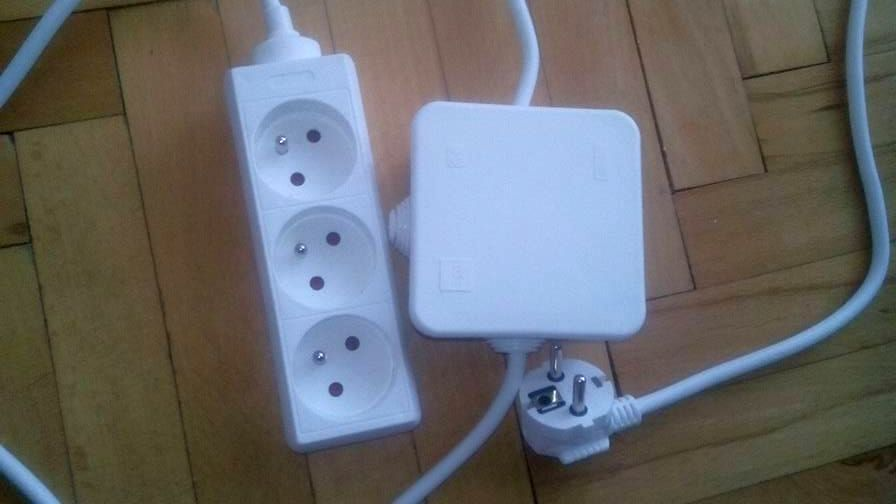
\includegraphics[width=1\hsize]{JPG/zestaw}
\caption{Zdjęcie złożonego zestawu}
\end{center}
\end{figure}

\newpage

Do działania aplikacji potrzebujemy przynajmniej jednej listwy z układem ESP  i dostępu do komputera. Podłączamy urządzenie do prądu, a na komputerze wystarczy wpisać w przeglądarce adres  http://192.168.1.186:8090, by znaleźć się na stronie głównej panelu obsługi naszego urządzenia. 

\hspace{2cm}
\begin{figure}[h]
\begin{center}
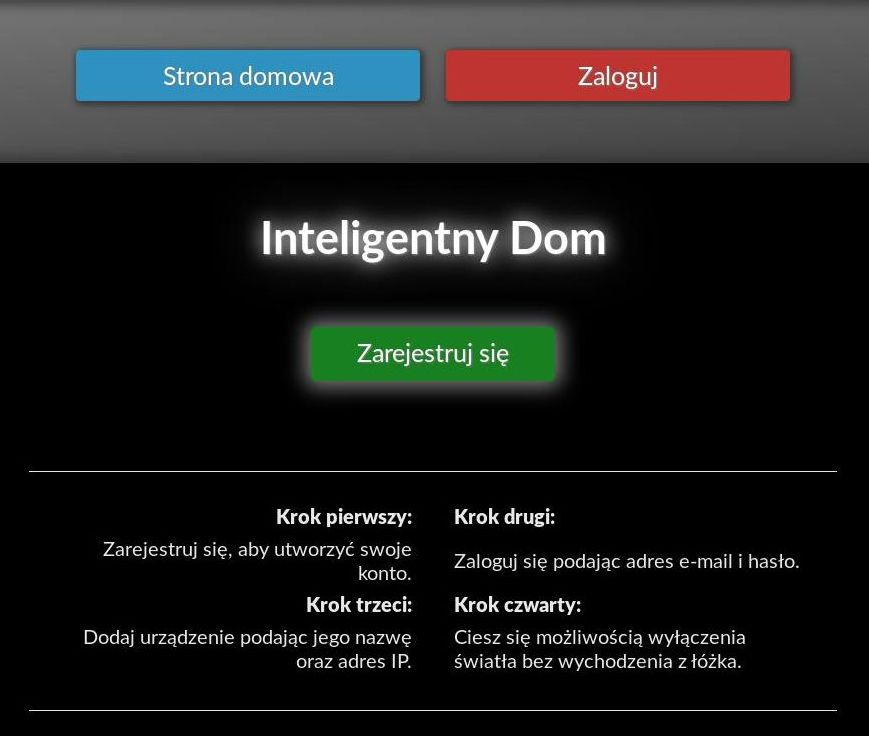
\includegraphics[width=0.8\hsize]{JPG/glowna}
\caption{Strona główna}
\end{center}
\end{figure}

Jeśli jesteśmy nowymi użytkownikami, najpierw trzeba się zarejestrować. W tym celu należy podać swój login, adres e-mail, hasło oraz numer telefonu. Na podany numer zostanie wysłany czterocyfrowy, losowy kod aktywacyjny, którym potwierdzimy swoją tożsamość i będziemy mogli zalogować się do panelu sterowania.

\begin{figure}
\begin{center}
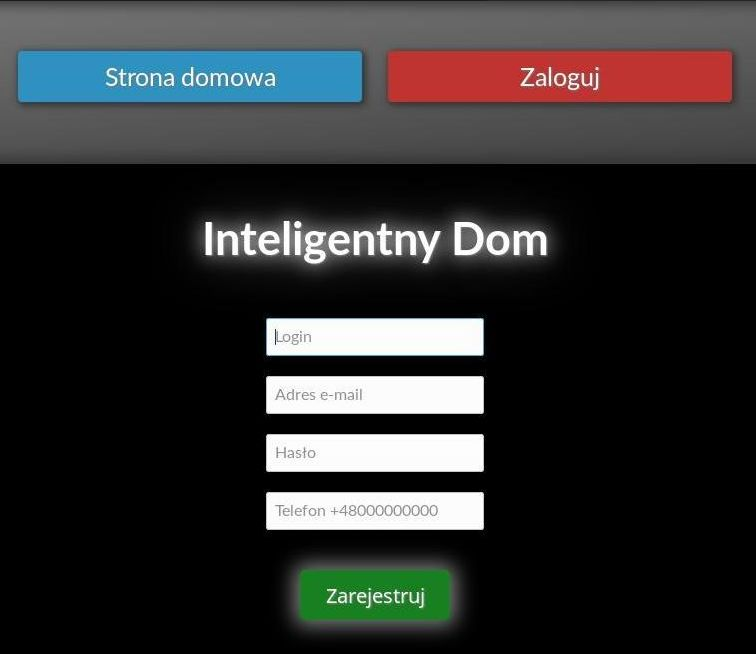
\includegraphics[width=0.75\hsize]{JPG/rejestr}
\caption{Rejestracja}
\end{center}
\end{figure}

\begin{figure}
\begin{center}
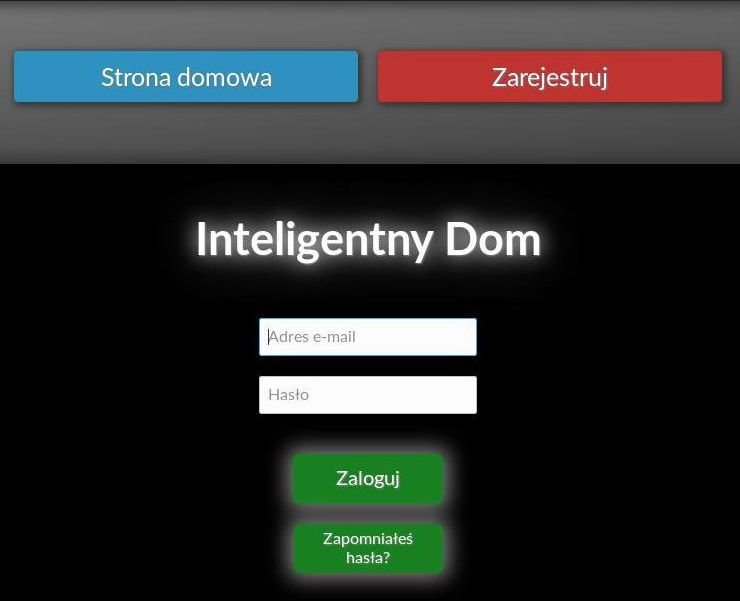
\includegraphics[width=0.75\hsize]{JPG/logow}
\caption{Logowanie}
\end{center}
\end{figure}

\newpage W przypadku gdy nasze hasło nie działa bądź go zapomnieliśmy, możemy wykorzystać funkcję  „Zapomniałeś hasła?”. Po wpisaniu adresu e-mail, wykorzystanego podczas rejestracji, ponownie otrzymamy czterocyfrowy kod, który umożliwi nam przejście do naszego panelu. Po zalogowaniu możemy zmienić hasło na nowe w zakładce „Zmień hasło”.

\hspace{2cm}
\begin{figure}[h]
\begin{center}
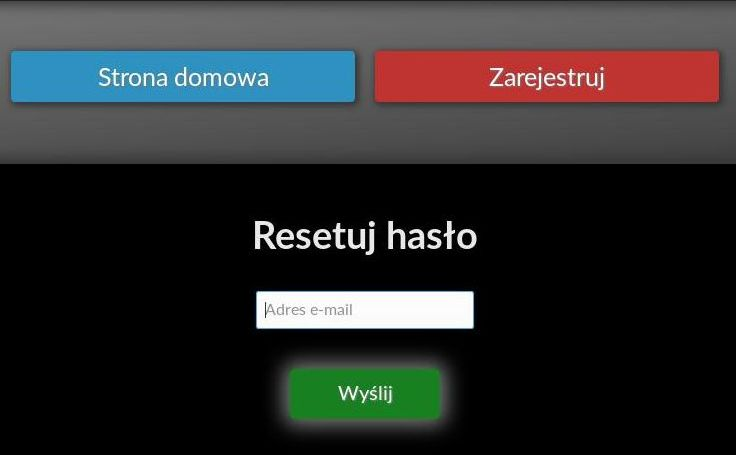
\includegraphics[width=0.8\hsize]{JPG/resethas}
\caption{Zmiana hasła}
\end{center}
\end{figure}


Początkowo panel starowania będzie pusty. Aby dodać do widoku układ, nad którym chcemy sprawować kontrolę, trzeba kliknąć przycisk „Dodaj urządzenie”, a kolejnej stronie, podać  wygodną dla nas nazwę (np. kuchnia) oraz adres IP, który został przekazany wraz z urządzeniem. W przypadku braku połączenia, wyświetli się błąd. W takiej sytuacji należy sprawdzić czy listwa z układem ESP otrzymuje zasilanie z gniazdka i czy podłączony do niej sprzęt działa prawidłowo. Następnie proszę powtórzyć próbę dodania urządzenia. 

\begin{figure}
\begin{center}
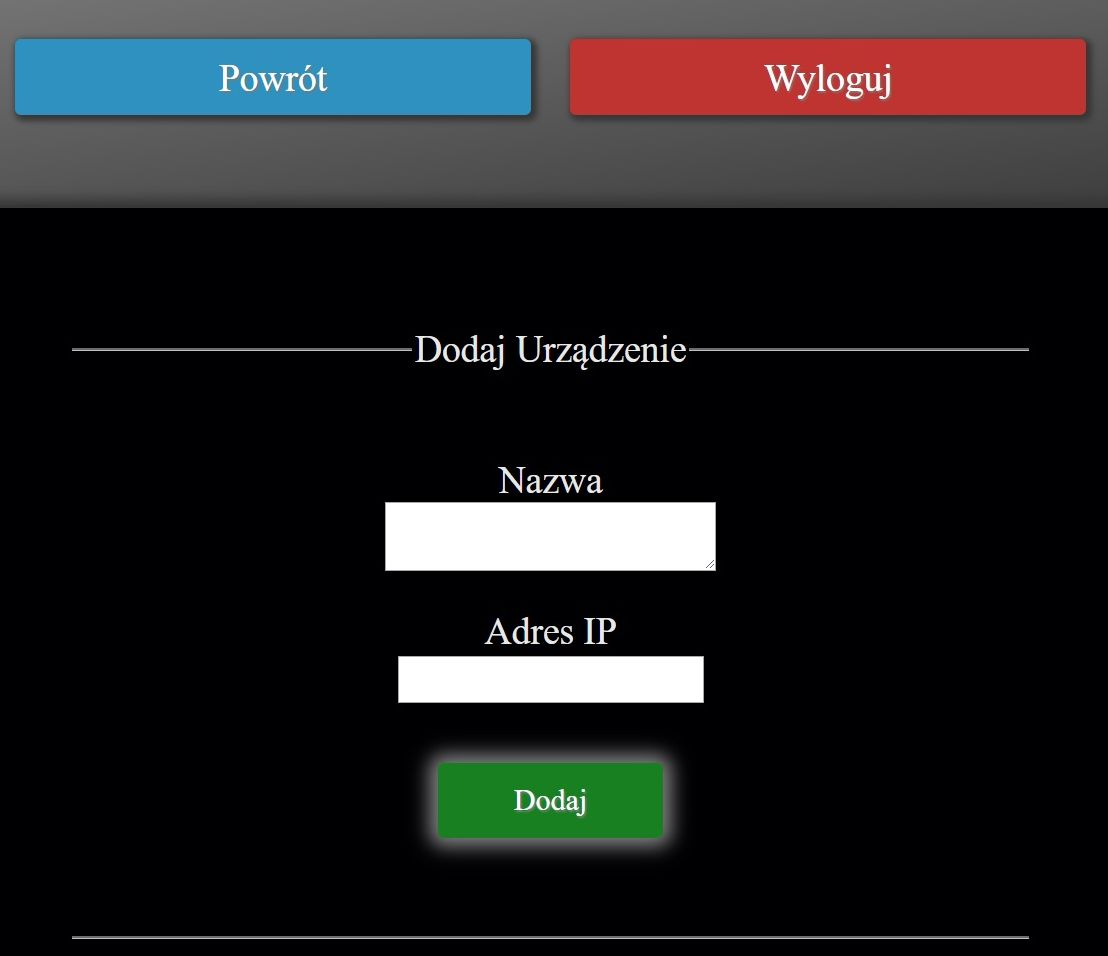
\includegraphics[width=0.8\hsize]{JPG/dodaj_urzadzenie}
\caption{Dodawanie urządzenia}
\end{center}
\end{figure}

\begin{figure}
\begin{center}
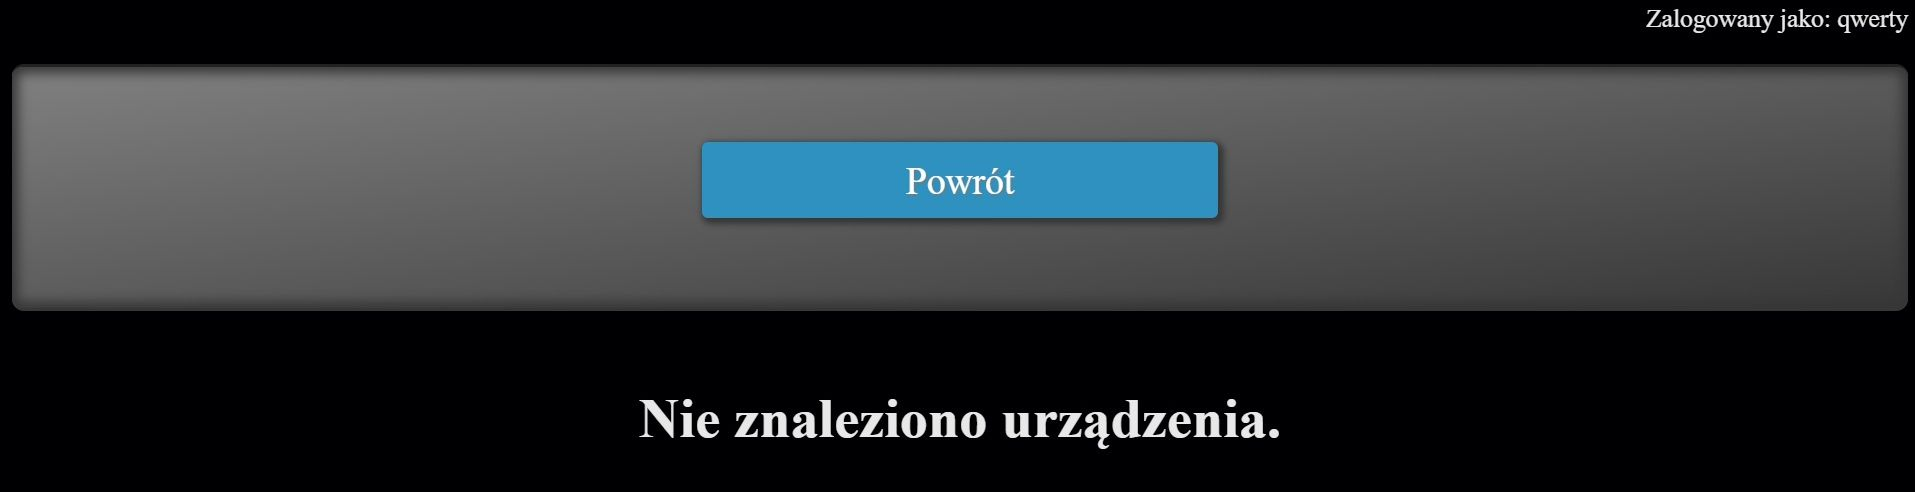
\includegraphics[width=0.8\hsize]{JPG/nie_zanleziono}
\caption{Komunikat błędu}
\end{center}
\end{figure}

\newpage Po przejściu wszystkich kroków, w panelu sterowania zobaczymy listę z dodanymi przez nas układami. Odczytamy tu podane wcześniej informacje o nazwie, adresie IP a także o stanie urządzenia. Gdy stan określony jest jako „Włączone”, poprzez kliknięcie przycisku „Wyłącz”, odcinamy dopływ prądu i wyłączamy nasz sprzęt, analogicznie w odwrotnym przypadku. W momencie gdy chcemy zmienić nazwę urządzenia lub po prostu usunąć je z listy, wystarczy kliknąć przycisk „Usuń” . Po otrzymaniu potwierdzenia przestanie ono być widoczne w panelu. W każdej chwili urządzenie można dodać ponownie. 

\hspace{2cm}
\begin{figure}[h]
\begin{center}
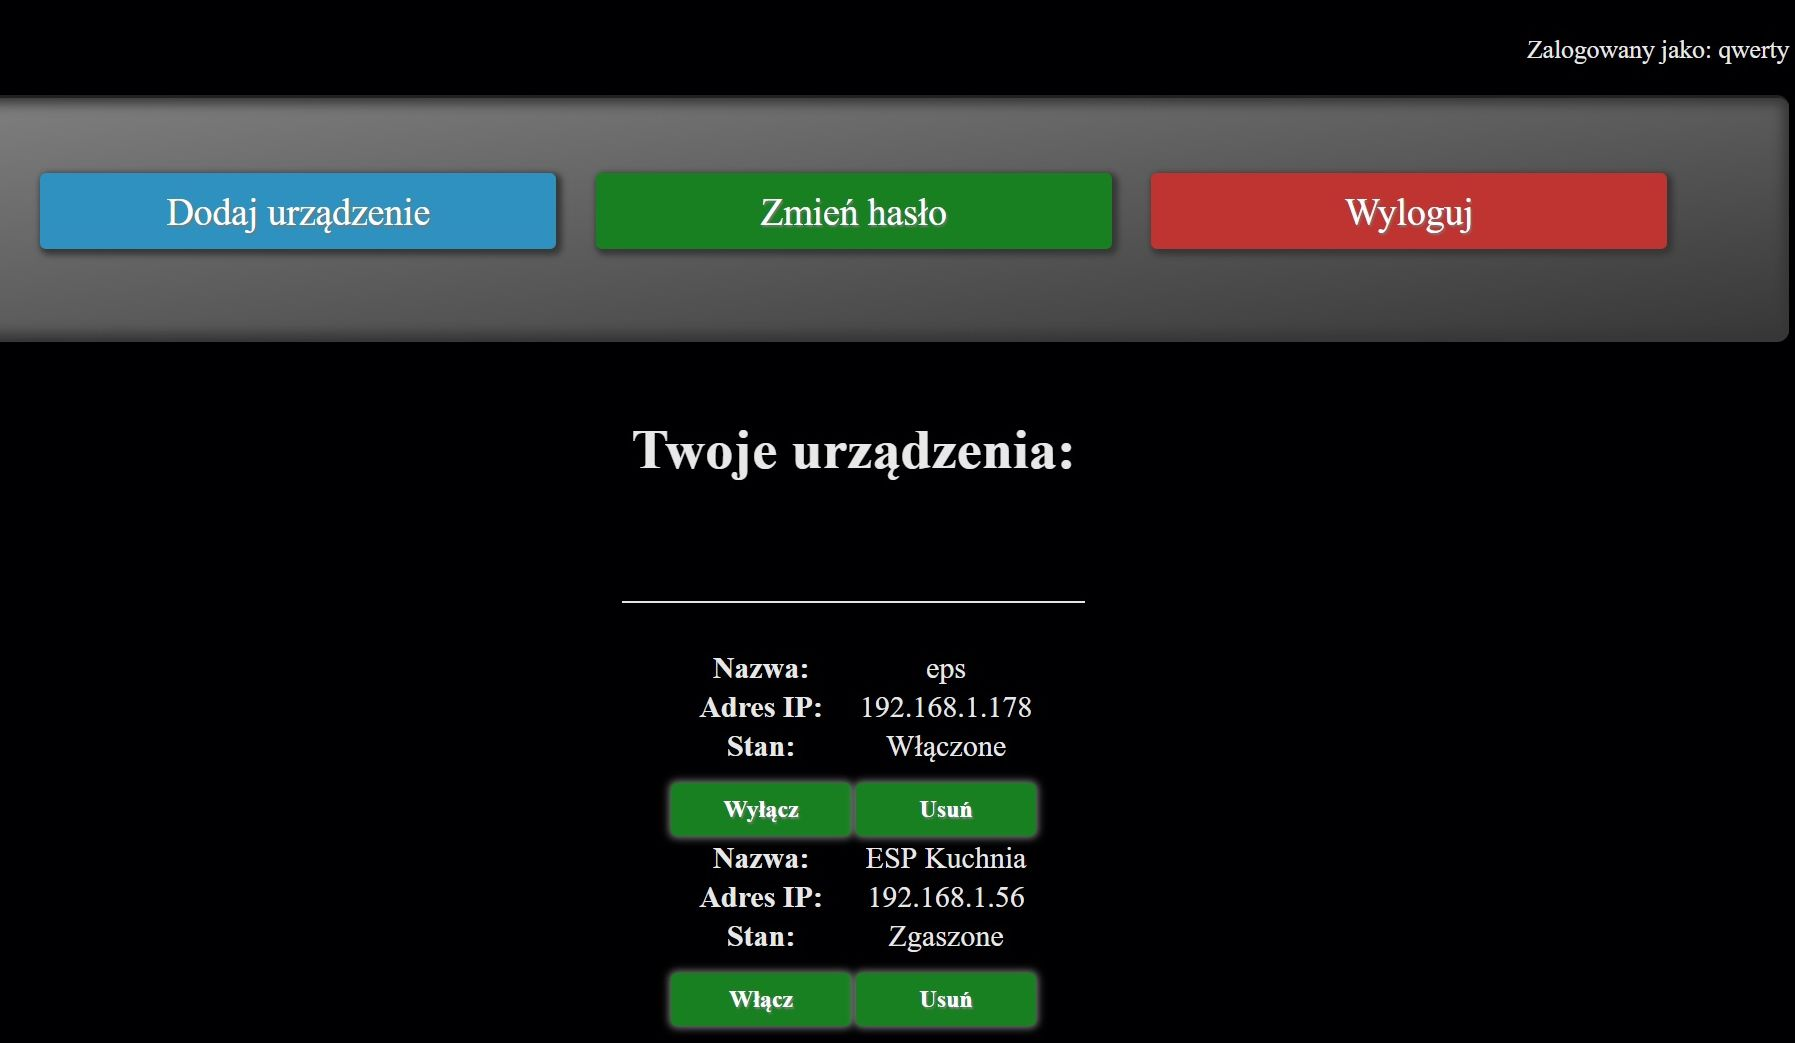
\includegraphics[width=1\hsize]{JPG/lista_urzadzen2}
\caption{Panel sterowania}
\end{center}
\end{figure}

\newpage Ogólny schemat działania aplikacji został przedstawiony na diagramie DFD:

\hspace{2cm}
\begin{figure}[h]
\begin{center}
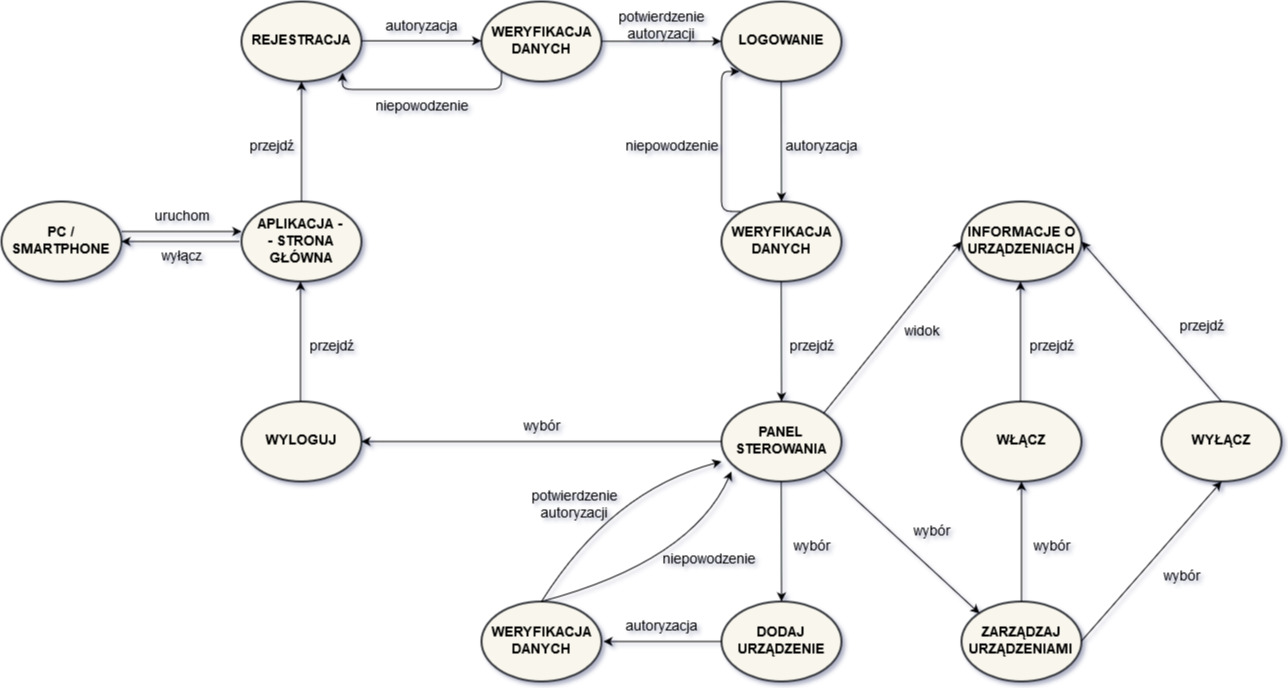
\includegraphics[width=1.1\hsize]{JPG/diagram}
\caption{Diagram DFD}
\label{Diagram}
\end{center}
\end{figure}

%%%%%%%%%%%%%%%%%%%%%%%%%%%        II  RODZIAŁ           %%%%%%%%%%%%%%%%%%%%%%%%%%%%%%%%%%%%%%%%%%%
\chapter{Mobile app}


%%%%%%%%%%%%%%%%%%%%%%%%%%%       podrozdział 2.1          %%%%%%%%%%%%%%%%%%%%%%%%%%%%%%%%%%%%%%%%%%%
\section{Kivy -- czym jest?}
Jest to biblioteka stworzona z myślą o interfesjach graficznych. Aplikację w której kivy zostało wykorzystane możemy uruchomić na 
Windowsie, Linuksie, MacOS, Androidzie oraz iOS. Istnieją dwie metody tworzenia GUI, z poziomu Pythona oraz Kvlang. Obie metody można ze sobą dowolnie łączyć. Sam Framework istnieje od niedawna, jest typem open source, wciąż rozwijanym i darmowym. Wydają go twórcy, którzy na codzień zajmują się właśnie dystrybucją oprogramowania na urządzenia mobilne. Zostali oni również zauważeni przez Python Software Fundation, którzy wsparli ich dotacją w 2012 roku, za port do Pythona3. Biblioteka podlega warunkom MIT.

%%%%%%%%%%%%%%%%%%%%%%%%%%%       podrozdział 2.2          %%%%%%%%%%%%%%%%%%%%%%%%%%%%%%%%%%%%%%%%%%%
\section{Dlaczego został wybrany?}
Jednym z przedmiotów podczas realizowania programu nauczania studiów I stopnia informatyki był właśnie Python. Ze względu na czytelność i klarowność jego kodu został wybrany na język przewodni w naszym projekcie. Jako, że Kivy jest tworzone w Pythonie, a to główna zaleta odnośnie alternatywnych rozwiązań, zdecydowaliśmy się właśnie na ten framework. Również zaletami jest łatwe i niestandardowe tworzenie wyglądu. Dokumentacja jest napisana w sposób czytelny, zrozumiały dla osób mających styczność pierwszy raz z Kivy. Problemem przede wszystkim może być to, że ta technologia jest dość „świeża”, co za tym idzie szukanie pomocy na forach kończy się praktycznie zerowym odzewem. Jeszcze jednym zauważalnym minusem okazuje się być narzędzie do „deploy'owania” - Buildozer, który działa poprawnie tylko na linuksie.

%%%%%%%%%%%%%%%%%%%%%%%%%%%       podrozdział 2.3          %%%%%%%%%%%%%%%%%%%%%%%%%%%%%%%%%%%%%%%%%%%
\section{Kivy ScreenManager}
Menadżer ekranu\footnote{https://kivy.org/docs/api-kivy.uix.screenmanager.html} jest to widżet posiadający funkcję zarządzania wieloma ekranami. Domyślnie, wyświetla tylko jeden ekran na raz i używa funkcji TransitionBase do przejścia do następnego widoku. Wiele z nich jest obsługiwana w oparciu o zmianę współrzednych ekranu, pozwala również na wykonywanie niestandardowych animacji za pomocą shaderów.
Poruszanie się po naszej aplikacji oparliśmy właśnie o ScreenMenager. Wykorzystaliśmy do tego przyciski(ang. button), za którymi kryje się funkcja odpowiadająca za komunikowanie się z widokiem napisanym w pliku kv. 

\begin{lstlisting}  [style=py] 
def login{self}:
	self.root.current = 'login'
\end{lstlisting}
Przykładowo prosta funkcja, która odwołuje się do naszego w tym wypadku podanego w cudzysłowie ID - login. Jeśli podane przez nas ID w funkcji istnieje w pliku kv, ScreenManager przeniesie nas w aplikacji do docelowego widoku. 
\begin{lstlisting}  
Screen:
	name:  'login'
\end{lstlisting}
Screen oznacza w tym wypadku rozpoczęcie nowego widoku i przypisania mu identyfikora. W naszym wypadku jest to login, aby w późniejszym rozbudowaniu aplikacji kod był przejrzysty i intuicyjny. 
\subsection{Komunikacja widoku z funkcją}
\begin{lstlisting}  
Button:
	text: 'Login'
	on_press: app.login()
	background_normal: 'button_normal.png'
	background_down: 'button_down.png'
\end{lstlisting}
W naszym widoku zdefininiowaliśmy przycisk. Posiada on pole typu text, gotową funkcję on\_press zaczerpnięta z framework'u, oraz wygląd zaimportowany z plików png. On\_press, jak sama nazwa wskazuje, po wciśnięciu wykona pożądane przez nas działanie. W tym wypadku, jeśli istnieje app.login zostanie wywołana funkcja.  
\subsection{Przykładowy screen}
\begin{lstlisting} 
Screen:
name: 'login'
GridLayout:
	label:
             id: username_label
	     text: 'Nazwa uzytkownika:'
	     TextInput:
	     id: username_input
	label:
             id: password_label
	     text: 'Hasło:'
	     TextInput:
	     id: password_input
             password: True
	Button:
	     text: "Zaloguj"
             on/_press: app.zaloguj()
	     background_normal: 'button_normal.png'
             background_down: 'button_down.png'		
	Button:
	     text: "Cofnij"
             on_press: app.cofnij()
	     background_normal: 'red_button_normal.png'
             background_down: 'red_button_down.png'
\end{lstlisting}
W pełni zdefiniowany

%%%%%%%%%%%%%%%%%%%%%%%%%%%       podrozdział 2.4          %%%%%%%%%%%%%%%%%%%%%%%%%%%%%%%%%%%%%%%%%%%
\section{Layout w Kivy}
W kivy tworzenie layout'u jest dość specyficzne. Jest kilka możliwości ułożenie naszych widżetów w określony sposób. Wyróżniamy:
\begin{itemize}
\item Anchor Layout mogą być zaczepione do górnego, dolnego, lewego, prawego boku lub do środka.
\item BoxLayout: ułożenie w orientacji pionowej lub poziomej.
\item FloatLayout: nieograniczony układ.
\item RelativeLayout: są rozmieszczane względem układu.
\item GridLayout: ułożone w „siatkę” zdefiniowaną przez rzędy i kolumny.
\item PageLayout: do tworzenia układów wielostronicowych, umożliwiający w łatwy sposób przewijanie z jednej strony na drugą.
\item ScatterLayout: podobnie jak w RelativeLayout, ale można je obracać i skalować.
\item StackLayout: ułożenie widżetów od lewej do prawej.
W naszej aplikacji wykorzystaliśmy GridLayout oraz BoxLayout.
\subsection{BoxLayout}
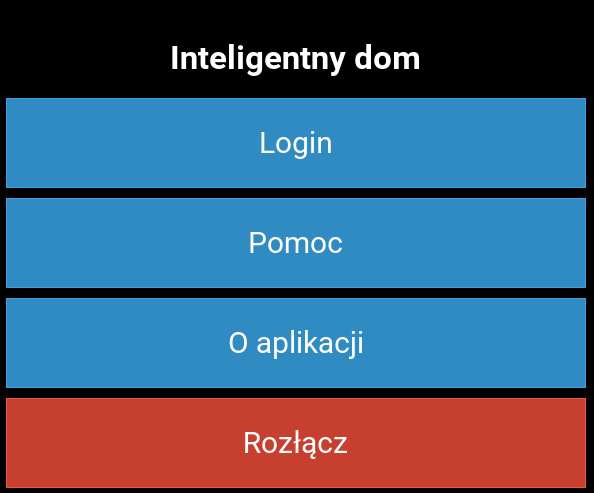
\includegraphics[width=0.8\hsize]{JPG/boxlayout} 
\newline
Tak wygląda nasze menu aplikacji mobilnej po podłączeniu się do serwera za pomocą framework'u Twisted. Jest ono zdefiniowane w wyżej wymienionym BoxLayout. Został ułożony on w orientacji pionowej. \newline Definiuje się to w następujący sposób:
\begin{lstlisting} 
BoxLayout:
   orientation: 'vertical'
\end{lstlisting}
\end{itemize}
Ważną kwestią w tworzeniu layout'u jest zaprogramowanie jego paremetrów. W tym wypadku najważniejszym będzie ustawienie odstępów między odstępami. Czyli:
\begin{lstlisting} 
<BoxLayout>:
	padding: 10
	spacing: 10
\end{lstlisting}
Przy czym padding jest wypełnieniem pozycji pomiędzy dwoma polami, a spacing odstępami podanymi w pikselach.
\subsection{GridLayout}
Przykład wykorzystania GridLayout w jednym z widoków.  Ułożenie 


%%%%%%%%%%%%%%%%%%%%%%%%%%%        III  RODZIAŁ           %%%%%%%%%%%%%%%%%%%%%%%%%%%%%%%%%%%%%%%%%%%
\chapter{Web app}

%%%%%%%%%%%%%%%%%%%%%%%%%%%       podrozdział 3.1          %%%%%%%%%%%%%%%%%%%%%%%%%%%%%%%%%%%%%%%%%%%
\section{Python - Flask -- co to takiego?}
„Python jest dynamicznie typowanym językiem interpretowanym wysokiego poziomu”\cite{Bednarz:2017:Python}. Oznacza to, że Pyhton jest wykonywany na bieżąco, linijka po linijce. Nie jest on kompilowany, a jedynie wczytywany i wykonywany podczas uruchomienia przez interpreter języka. Języki skryptowe są mniej wydajne od języków kompilowanych, jednakże są dość proste w użyciu, przez co dobrze sprawdzają się podczas pisania niewielkich aplikacji. 
Podstawowymi framework’ami\footnote{\url{https://pl.wikipedia.org/wiki/Framework}} Python’a są Django oraz Flask\cite{Ronacher:2017:Flask}. Naszym założeniem było stworzenie prostej i szybkiej aplikacji, dlatego zdecydowaliśmy się na wykorzystanie Flask’a. Jest to micro-framework obsługujący rozszerzenia, które mogą dodawać funkcje do aplikacji, takie jak sprawdzanie poprawności formularzy, obsługa wysyłania czy otwarte technologie uwierzytelniania. Ponadto jest kompatybilny z Google App Engine, zawiera zintegrowaną obsługę testów jednostkowych, obsługę plików cookie, a przede wszystkim posiada serwer programistyczny i debugger. Dzięki temu nie wymaga żadnych dodatkowych narzędzi. Dzięki swoim funkcjom, Flask upraszcza projektowanie stron www. 

%%%%%%%%%%%%%%%%%%%%%%%%%%%       podrozdział 3.2          %%%%%%%%%%%%%%%%%%%%%%%%%%%%%%%%%%%%%%%%%%%
\section{Zastosowanie w aplikacji}
Serce naszej aplikacji, główny kod i schemat działania, zawarty jest w czterech podstawowych plikach: run.py, model.py, views.py oraz \newline\_\_init\_\_.py.  Pierwszy plik określa ścieżkę do serwera, drugi odpowiada za komunikację z bazą danych a trzeci za wyświetlanie i zachowanie stron internetowych. Plikiem, bez którego działanie aplikacji nie byłoby możliwe jest \_\_init\_\_.py. Plik ten odpowiada za import klas bądź funkcji do poziomu pakietu, aby można je było wygodnie importować w późniejszym etapie. Flask używa nazwy „import”, aby wiedzieć, gdzie szukać zasobów, szablonów, plików statycznych, folderu instancji, itp.
Komendy:
\begin{lstlisting} [style=py] 
from flask import Flask
from flask_sqlalchemy import SQLAlchemy
from flask_login import LoginManager
\end{lstlisting}

umożliwiają nam korzystanie z samego Flask’a oraz zaimportowanie rozszerzeń SQLAlchemy oraz LoginManager, a polecenia takie jak 
\begin{lstlisting} [style=py] 
from www.model import baza, login_manager  
from www import views
\end{lstlisting}
odpowiadają za wskazanie lokalizacji powiązanych plików, z kolei 
\begin{lstlisting}  [style=py] 
app = Flask(__name__)
\end{lstlisting}
wskazuje na miejsce przechowywania zasobów aplikacji. 

\subsection{Flask -- SQLAlchemy}

SQLAlchemy jest stworzonym dla Pythona narzędziem,  który wraz z ORM\footnote{Object Relational Mapper} oferuje pełną funkcjonalność języka SQL bez konieczności samodzielnego pisania skomplikowanych zapytań. Flask-SQLAlchemy z kolei jest niczym innym jak rozszerzeniem dodającym usługę SQL do programu. 

W naszym przypadku do pełnego i bezpiecznego działania aplikacji, konieczne było stworzenie tabel przechowujących dane logujących się osób oraz informacje o podłączanych urządzeniach.
Aby nasza baza mogła funkcjonować w pliku \_\_init\_\_.py utworzyliśmy jej instancję 

\begin{lstlisting}  [style=py] 
baza.init_app(app)
app.static_folder = 'static'
baza.app = app
baza.create_all()
\end{lstlisting}

by w pliku model.py móc zadeklarować tabele „User” oraz „Esp”

\label{Model}
\begin{lstlisting}  [style=py] 
class User(baza.Model, UserMixin):
    id = baza.Column('id', baza.Integer, primary_key=True)
    imie = baza.Column('imie', baza.String)
    email = baza.Column('email', baza.String, unique = True)
    haslo = baza.Column('haslo', baza.String)
    telefon = baza.Column('telefon', baza.String)
    aktywne = baza.Column('aktywne', baza.Boolean, default=False)
    pin = baza.Column('pin', baza.Integer)
    def __init__(self, imie, email, haslo, telefon, aktywne, pin):
        self.imie = imie
        self.email = email
        self.haslo = self.hash_password(haslo)
        self.telefon = telefon
        self.aktywne = aktywne
        self.pin = pin
        def __repr__(self):
            return ('<User %r>' % self.email)
    
    def hash_password(self, password):
        return pwd_context.encrypt(password)
    
    def verify_password(self, password):
        return pwd_context.verify(password, self.haslo)
\end{lstlisting}

\begin{lstlisting}  [style=py] 
class Esp(baza.Model):
    id = baza.Column('id', baza.Integer, primary_key=True)
    nazwa = baza.Column('nazwa', baza.String)
    ip = baza.Column('ip', baza.String)
    stan = baza.Column('stan', baza.Boolean, default=False)
    def __init__(self, nazwa, ip, stan):
        self.nazwa = nazwa
        self.ip = ip
        self.stan = stan
\end{lstlisting}

Jak widać nie stosowaliśmy tu klasycznego zapisu języka SQL, a każda tabela powstała jako klasa, w której deklarujemy poszczególne kolumny i ich właściwości. Funkcje "def \_\_init\_\_" służą przypisaniu odpowiednich wartości, z kolei "def hash\_password" oraz "def verify\_password" są wbudowanymi funkcjami Python’a, wykorzystanymi do podniesienia poziomy bezpieczeństwa poprzez zaszyfrowanie hasła wpisywanego przez użytkownika, oraz jego weryfikacjię podczas logowania. Wszelkie dane pobierane od użytkownika, przesyłane są za pomocą metod „GET” i „POST”. W pliku view.py, poprzez tzw. dekoratory deklarujemy powiązanie funkcji z adresem URL. Na przykład w przypadku próby zarejestrowania się, kliknięcie przycisku „Zarejestruj” wywoła funkcję „def register”.

\begin{lstlisting}  [style=py] 
@app.route('/register', methods = ['GET', 'POST'])
def register():
    if request.method == 'POST':
        ...
        uzytkownik = User(imie=request.form['imie'], email=request.form['email'], haslo=request.form['haslo'], telefon=telefon, aktywne = 0, pin=pin )
        ...
        return redirect(url_for('autoryzacja'))
    return render_template('signup.html')
\end{lstlisting}

Funkcja ta w przypadku poprawnego przekazania danych, generuje losowy kod weryfikacyjny, zapisuje informacje uzyskane do użytkownika do bazy danych poprzez zmienną „użytkownik”, następnie wywołuje funkcję oraz stronę odpowiedzialne za autoryzację kodu aktywacyjnego i w przypadku wykonania wszystkich zadań z powodzeniem, przekierowuje nas na stronę logowania. Jak widać samo zapytanie SQL przekazujące informacje odbywa się przez „request.form” i nie zajmuje więcej niż jedną linijkę kodu, dzięki czemu możemy skupić się na budowaniu innych funkcji.

\subsection{Flask -- LoginManager}
Flask – LoginManager\cite{Frazier:2018:flask} jest narzędziem umożliwiającym zarządzanie sesją użytkownika poprzez obsługę zadań takich jak logowanie, wylogowywanie czy zapamiętywanie identyfikatora użytkownika w sesji. Aby móc korzystać z tych funkcji należy najpierw stworzyć model użytkownika o właściwościach: 

\newpage
\begin{lstlisting} [style=py] 
@property
def is_authenticated(self):
    return True
@property       
def is_active(self):
    return True
def is_anonymous(self):
    return False
def get_id(self):
   	return str(self.email)
\end{lstlisting}

Odpowiadają one za weryfikację czy klient podał prawidłowe poświadczenia, czy jego konto jest aktywne oraz czy bieżący użytkownik jest anonimowy. Metoda get\_id bierze pod uwagę instancję klasy User \ref{Model} i zwraca unikalny numer dla tego obiektu. Identyfikator użytkownika jest brany pod uwagę w funkcji „user\_loader”:

\begin{lstlisting} [style=py] 
@login_manager.user_loader
def load_user(user_id):
    return User.query.get(int(user_id))
\end{lstlisting}

Ma ona za zadanie przekazać programowi z jakim użytkownikiem będzie pracował i jakie dane ma wyświetlić. 

Proces logowania odbywa się z kolei w funkcji „login”:

\begin{lstlisting} [style=py] 
@app.route('/login', methods = ['GET', 'POST'])
def login():
    if request.method == 'POST':
        haslo = request.form['haslo']
        mail = request.form['email']
        user=User.query.filter(User.email==mail).first()
        if user:
            if user.verify_password(haslo) == True:
                if user.aktywne == 1:
                    login_user(user, remember=True)
                    return redirect(url_for('list_all'))             
                return redirect(url_for('autoryzacja'))
            return render_template('error.html',error = 'Haslo niepoprawne.')
        return render_template('error.html',error = 'Nie ma takiego konta.')       
    return render_template('signin.html')
\end{lstlisting}

Adres e-mail oraz hasło przekazywane są za pomocą metod „GET” i „POST”. W pierwszej kolejności  polecenie „User.query.filter(User.email==mail). first()” wyszukuje w bazie użytkownika o podanym adresie e-mail, by kolejno, zweryfikować poprawność wprowadzonego hasła, sprawdzić czy konto użytkownika zostało aktywowane oraz by pobrać i zapamiętać jego identyfikator dla bieżącej sesji. W przypadku jakiegokolwiek błędu otrzymamy komunikat bądź zostaniemy przekierowani na odpowiednią stronę. 

Przed wywołaniem każdej funkcji, która ma za zadanie wyświetlać lub przekazywać prywatne informacje, skorzystaliśmy z dekoratora „login\_required”. Ma on za zadanie zapewnić poprawność wyświetlanych informacji dla danego użytkownika oraz uniemożliwić dostęp osobom niepowołanym. Na przykład przed funkcją przekierowującą do strony panelu sterowania:

\begin{lstlisting} [style=py] 
@app.route('/wyswietl')
@login_required
def list_all():
    esp=Esp.query.all()
    return render_template('showDevices.html', esp = esp)
\end{lstlisting}

%%%%%%%%%%%%%%%%%%%%%%%%%%%       podrozdział 3.3          %%%%%%%%%%%%%%%%%%%%%%%%%%%%%%%%%%%%%%%%%%%
\section{Autoryzacja SMS}
Użytkownik, który stworzył konto w naszej aplikacji, przy pierwszym logowaniu musi wykonać jednorazową autoryzację konta za pomocą kodu PIN, który otrzymał w formie SMS'a\footnote{ang. \emph{Short Message Service}}. Kod PIN generowany jest 
wbudowaną funkcją Pythona "random":
\begin{lstlisting} [style=py] 
pin = random.randint(1000,9999)
\end{lstlisting}
Kod zostaje przypisany użytkownikowi i zapisany bazie danych.

Wysłanie wiadomości tekstowej na wskazany przy rejestracji nr telefonu odbywa się przez modem GSM oraz funkcję „wyslijsms”:
\begin{lstlisting} [style=py] 
def wyslij_sms(numer, pin):
    text = pin
    number = numer
    s = serial.Serial('/dev/ttyUSB2', 115200, timeout=1)
    s.write(bytes('AT\r', 'UTF-8'))
    time.sleep(1)
    msg=s.read(64)
    print(msg)
    s.write(bytes('AT+CMGF=1\r', 'UTF-8'))
    time.sleep(1)
    msg=s.read(64)
    print(msg)
    s.write(bytes('AT+CMGS="%s"\r' % number, 'UTF-8'))
    #Send message:
    time.sleep(1)
    msg=s.read(64)
    print(msg)
    s.write(bytes('%s\x1a' % text, 'UTF-8'))
    msg=s.read(64)
    print(msg)
    s.close()
    return 0
\end{lstlisting}

Komunikacja aplikacji i modumu GSM odbywa się przez komendy AT\footnote{\url{https://sonnguyen.ws/send-sms-from-raspberry-pi-with-usb-3g/}} oraz bibliotekę PySerial 3.4\footnote{\url{http://pyserial.readthedocs.io/en/latest/pyserial.html}}

%%%%%%%%%%%%%%%%%%%%%%%%%%%       podrozdział 3.4          %%%%%%%%%%%%%%%%%%%%%%%%%%%%%%%%%%%%%%%%%%%
\section{Tworzenie stron internetowych}
Przy projektowaniu aplikacji internetowej posłużyliśmy się językiem \newline HTML\cite{seo:2011:SEO}\footnote{ang. \emph{HyperText Markup Language }} służącym do umieszczania treści na stronie oraz CSS\cite{w3c:2018:css}\footnote{ang. \emph{Cascading Style Sheets }} odpowiadającym za formatowanie jej wyglądu. Oba języki są proste w użyciu,  a co najważniejsze, dzięki swojej popularności wspierane większość przeglądarek internetowych. Jedyną wadą jest różne działanie arkuszy stylów na poszczególnych przeglądarkach, jednakże zasady ich działania są proste i przy zachowaniu odpowiednich reguł, nie musimy obawiać się niepoprawnego wyświetlania treści naszej strony. W sieci istnieje wiele gotowych (darmowych bądź płatnych) arkuszy, które możemy pobrać i zaimportować do swojego projektu, dzięki temu oszczędzimy swój czas, a strona będzie wyglądać bardziej profesjonalnie. 

W przypadku naszego projektu korzystanie z gotowych szablonów nie było konieczne. Z założenia strona wyglądem miała być zbliżona do aplikacji mobilnych, które cechuje dość prosty design w kontrastowych barwach, aby dobrze prezentowały się na małym wyświetlaczu telefonu.

Podstawą zasadą przy tworzeniu stron HTML jest trzymanie się ogólnych norm przyjętych przez W3C\footnote{\url{https://pl.wikipedia.org/wiki/World_Wide_Web_Consortium}}. Przy dbaniu o przejrzystość kodu, poprawnym stosowaniu znaczników oraz atrybutów, dopisanie do naszej strony arkusza stylu nie powinno sprawić większych problemów. Za powiązanie języka CSS z HTML’em odpowiedzialne są tzw. selektory, którymi mogą być elementy HTML oraz atrybuty „id” oraz „class”. Przykładem w naszej pracy może być określenie wyglądu przycisków „Dodaj” bądź „Wyślij”.

\hspace{2cm}
\begin{figure}[h]
\centering
\subfloat{

\includegraphics[width=0.4\textwidth]{JPG/dadaj}}
\quad
\subfloat{

\includegraphics[width=0.4\textwidth]{JPG/wyslij}}
\quad
\caption{Przyciski na stronach "Dodaj urządzenie" oraz "Zmień hasło"}
\end{figure}

\begin{lstlisting} [style=py]
<div>
	<input class="button" type = "submit" value = "Wyslij" />
</div>

<div>
	<input class="button" type = "submit" value = "Dodaj" />
</div>
\end{lstlisting}

\begin{lstlisting} [style=py]
.button {
  margin-top: 20px;
  height: 50px;
  width: 150px;
  cursor: pointer;
  background-color: #188021;
  border: 2px solid #188021;
  color: white;
  font-size: 20px;
  font-weight: 400;
  border-radius: 4px;
  box-shadow: 0px 0px 20px 6px grey;
  text-shadow:1px 1px 1px grey;
}
.button:hover {
  color: #188021;
  background-color: #E8FFE9;
}
\end{lstlisting}

Mamy tutaj przykład dwóch przycisków opisanych atrybutami „value”, „type” i „class”. Pierwszy określa etykietę przycisku, drugi rodzaj wstawianego pola, a trzeci jest odwołaniem do pliku .css. Selektor „button” w naszym arkuszy stylu określa m.in. rozmiar przycisku (height, width), wygląd czcionki (color, font-size, font-weight. text-shadow), tła (background-color) czy nawet zaokrąglenia rogów (border-radius). Klasa „button:hover” z kolei odpowiada za zachowanie przycisku po najechaniu na niego myszką, w tym przypadku jego kolor i czcionka ulegną zmianie na przeciwne. 

 Obecnie treść przeglądarek internetowych możemy wyświetlać nie tylko na komputerach ale i telewizorach, projektorach, czytnikach e-book’ów oraz telefonach. W zależności od rozmiaru ekranu treść naszej strony może się nie zmieścić lub zostać rozciągnięta. Dlatego wraz w wprowadzeniem nowej wersji CSS3 zostały rozbudowane reguły @media. Dzięki nim możemy zmienić wygląd naszej strony w zależności na jakim urządzeniu zostanie wyświetlona. Nasza strona została dostosowana do małych ekranów telefonów (poniżej 730px) tak, aby elementy na niej zawarte dostosowały swoją pozycję. 

\hspace{2cm}
\begin{lstlisting} [style=py]
@media only screen and (min-width: 730px) {
  .footer {
    padding-right: 0;
    padding-left: 0;
  }
  .header {
    margin-bottom: 30px;
  }
  .jumbotron {
    border-bottom: 0;
  }
}
\end{lstlisting}


%%%%%%%%%%%%%%%%%%%%%%%%%%%       IV ROZDZIAŁ          %%%%%%%%%%%%%%%%%%%%%%%%%%%%%%%%%%%%%%%%%%%
\chapter{Hardware\label{PRZEGLAD.NARZEDZI}}

%%%%%%%%%%%%%%%%%%%%%%%%%%%       podrozdział 4.1          %%%%%%%%%%%%%%%%%%%%%%%%%%%%%%%%%%%%%%%%%%%
\section{ESP8266}
W naszym projekcie wykorzystalimy moduł WiFi oparty na układzie ESP8266-12E\footnote{\url{http://www.kloppenborg.net/images/blog/esp8266/esp8266-esp12e-specs.pdf}} jako sterownik przekaźnika. 
\hspace{2cm}
\begin{figure}[h]
\centering
\subfloat{
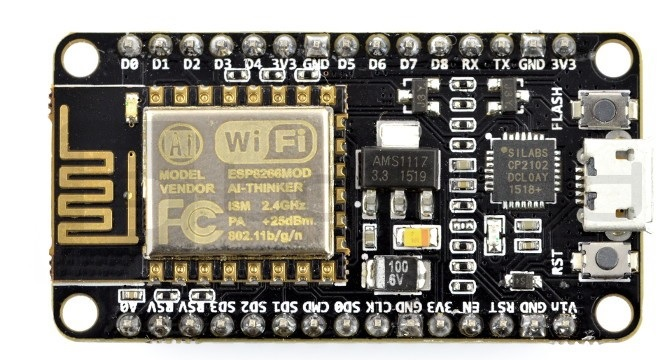
\includegraphics[width=0.3\textwidth]{JPG/ESP8266}}
\quad
\subfloat{
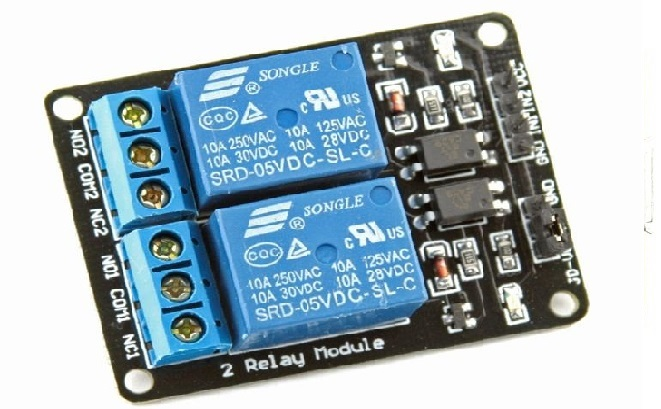
\includegraphics[width=0.3\textwidth]{JPG/przekaznik}}
\quad
\caption{Moduł ESP8266 i Przekaźnik 2-kanałowy}
\end{figure}

Esp Nodemcu v2 to programowalny mikrokontroler posiadający 32-bitowy CPU, 4MB pamięci Flash oraz 16 wyprowadzeń GPIO. Komunikacja odbywa się przez WiFi 802.11 b/g/n na częstotliwości 2,4 GHz. Do programowania układu wykorzystałem język "C" i środowisko Arduino IDE\footnote{\url{https://www.arduino.cc/en/main/software}}. Programator UART, który jest wlutowany w płytkę ułatwia wygrywanie programów przez standardowy kabel USB. 

ESP8266 został zaprogramowany do działania w trybie klienta WiFi w naszej lokalnej sieci. Dane dla naszej sieci podajemy przy programowaniu urządzenia:
\begin{lstlisting} [style=py] 
char* ssid = "NawaSieci";
char* pass = "HasłoSieci";

void setup() {
  WiFi.begin(ssid, pass);
}
\end{lstlisting}
Od tej chwili sterownik jest podłączony do routera.

Przekaźnik, który włącza lub wyłącza wysokie napięcie wyposażony jest w optoizolację\footnote{\url{https://pl.wikipedia.org/wiki/Transoptor}} zapewniając odseparowanie napięcia 230V a ESP8266. 

%%%%%%%%%%%%%%%%%%%%%%%%%%%       podrozdział 4.2          %%%%%%%%%%%%%%%%%%%%%%%%%%%%%%%%%%%%%%%%%%%
\section{Raspberry pi 3 - jako serwer aplikacji}
Mikrokomputer wyposażony w czterordzeniowy procesor ARM, 1 GB RAM, porty USB oraz HDMI. Cało pod kontrolą Linuxa specjalnie przygotowany dla Raspberry Pi 3\footnote{\url{http://docs-europe.electrocomponents.com/webdocs/14ba/0900766b814ba5fd.pdf}}. Zasilany przez 5V ładowarkę np. telefoniczną. Taką konfigurację posiada nasz serwer, który obsługuję  aplikację webową.
\hspace{2cm}
\begin{figure}[h]
\centering
\subfloat{
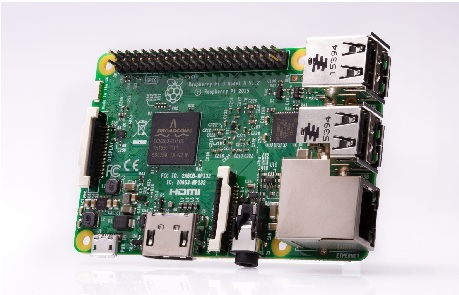
\includegraphics[width=0.4\textwidth]{JPG/rpi3.jpg}}
\quad
\caption{Raspberry Pi 3}
\end{figure}

%%%%%%%%%%%%%%%%%%%%%%%%%%%       podrozdział 4.3          %%%%%%%%%%%%%%%%%%%%%%%%%%%%%%%%%%%%%%%%%%%
\section{Komunikacja}
Raspberry Pi 3 i Esp8266 komunikują się ze sobą za pomocą pomocą JSON'ów. Gdy klient postawowi włączyć/wyłączyć urządzenie za pomocą ESP wywołuje funkcje na RPI 3 "swiatloon" lub "swiatlooff". Obie funkcje działają w identyczny sposób,  jedyną rożnicą jest wartosć pola "stan1" dla GPIO ESP generowanego JSONa. Funkcja "swiatloon" wygląda następująco:
\begin{lstlisting} [style=py] 
def swiatloon(idd):
    esp = session.query(Esp).filter(Esp.id ==int(idd)).one()
    conn = http.client.HTTPConnection(esp.ip)
    payload = "{\"stan1\":\"1\"}"
    headers = {
        'content-type': "application/json",
        }
    conn.request("POST", "/relay", payload, headers)
    res = conn.getresponse()
    data = res.read()
    return redirect(url_for('list_all'))
\end{lstlisting}
Pod zmienną \texttt{esp} zostaje przypisany obiekt ESP wyfiltrowany po ID. W \texttt{playload} przechowujemy stan GPIO do wysłania. Za samo przesłanie JSON'a na odpowiednie IP ESP odpowiada linia kodu \texttt{conn.request("POST", "/relay", payload, headers} oraz biblioteka http.client. 

Na adres 192.168.1.56/relay trafia pakiet danych z serwera RPI 3. ESP również jest serwerem, który przetwarza dane za pomocą funkcji:
\begin{lstlisting} [style=py] 
void setRelay() {

  String data = server.arg("plain");
  StaticJsonBuffer<200> jBuffer;
  JsonObject& jObject = jBuffer.parseObject(data);
  String stan1 = jObject["stan1"];
  int value1;
  String stanJson;
  value1=(stan1.toInt());
  if (value1==1){
      digitalWrite(pin, LOW);
      Serial.println(stan1);
       stanJson= "1";
  }
  else{
      digitalWrite(pin, HIGH);
      Serial.println(stan1);
      stanJson= "0";
  }
  StaticJsonBuffer<200> JSONbuffer;  
  JsonObject& JSONencoder = JSONbuffer.createObject();
  String ip = WiFi.localIP().toString();
  short int port = 8090;
  JSONencoder["ip"] = (ip);
  JSONencoder["stan"] = stanJson;
    char JSONmessageBuffer[200];
    JSONencoder.prettyPrintTo(JSONmessageBuffer, sizeof(JSONmessageBuffer));
    Serial.println(JSONmessageBuffer);
    HTTPClient http;    
    String adres="http://";
    adres+="192.168.1.186";
    adres+=":";
    adres+=port;
    adres+="/readjson";
    Serial.println();
    Serial.println(adres);
    http.begin(adres);      
    http.addHeader("Content-Type", "application/json");  
    int httpCode = http.POST(JSONmessageBuffer);   
    String payload = http.getString();                                        
    Serial.println(httpCode);  
    Serial.println(payload);    
    http.end();
    server.send(200,"ok");
}
\end{lstlisting}
Po odczytaniu wartosci \texttt{stan1} Esp zmienia stan pinu, czyli włącza prąd na danym porcie i uruchamia przekaźnik. Dalszy kod funkcji jest odpowiedzialny za odesłanie do serwera odpowiedzie w formie JSON'a z obcnym stanem urządzenia i jego IP. Dopiero, gdy serwer otrzyma odpowiedź na \texttt{/readjson} wraz z numerem ip i stanem goldpinu 8266, aktualizuje bazę danych: 
\begin{lstlisting} [style=py] 
@app.route('/readjson', methods=['POST'])
def readjson():
    print(request.is_json)
    content = request.get_json()
    print(content)
    ip = content["ip"]
    stan = content["stan"]
    print(stan, ip)
    esp = session.query(Esp).filter(Esp.ip ==ip).one()
    esp.stan = int(stan)
    session.commit()
    return redirect(url_for('list_all'))
\end{lstlisting}

%%%%%%%%%%%%%%%%%%%%%%%%%%%       podrozdział 4.4          %%%%%%%%%%%%%%%%%%%%%%%%%%%%%%%%%%%%%%%%%%%
\section{Bezpieczeństwo w projektach "Smart Home"}

Sieć Internetu Rzeczy i same urządzenia przetwarzają dane o naszej codziennej aktywności dobowej, np. kiedy włączamy światło. Po dłuższej analizie takich zachowań określić, czy jesteśmy w domu, na jak długo go opuszczamy lub kiedy do niego wracamy. Informacje takie jeśli dostaną się w niepowołane ręce mogą posłużyć do fizycznego włamania do naszego mieszkania.

Każde urządzenie w naszej sieci Internetu Rzeczy może być potencjalnym punktem włamania do infrastruktury IOT i ujawnieniem wrażliwych danych. Poprawą bezpieczeństwa może pomóc nam Blockchain. Technologia ta opiera się o sieć peer-to-peer. Czynności odbioru lub nadaniu danych przez urządzenie jest rozgłaszane w sieci przez co klienci rejestrują je w swoich blokach i zapisują w księdze transakcji. Bloki takich informacji zostają zapieczętowane. Do zapieczętowania wykorzystywane są poprzednie bloki, dzięki czemu próba manipulacji na jednym bloku powoduję dezintegrację całości.
\begin{figure}[h]
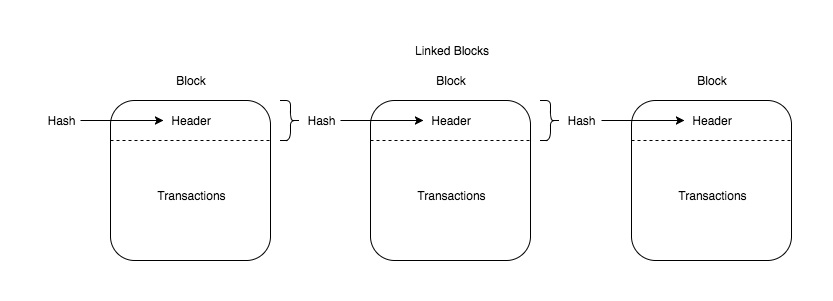
\includegraphics[width=1\textwidth]{JPG/blocks.jpg}
\caption{Pieczętowanie bloków}
\end{figure}

Wykorzystanie technologii Blockchain w sieci IOT ogranicza ryzyko włamań przez redukcję centralnych systemów autoryzacji, łatwą weryfikację danych oraz niezmienność.

zródło obrazku 4,4\footnote{\url{https://www.pluralsight.com/guides/blockchain-architecture}}

do bibliografii\footnote{\url{https://www.intel.pl/content/www/pl/pl/it-managers/the-benefits-of-blockchain-iot-biot.html}}

do bibliografii\footnote{\url{https://www.ibm.com/blogs/blockchain/2018/01/why-blockchain-and-iot-are-best-friends/}}

do bibliografii\footnote{\url{https://blog.kurasinski.com/2017/07/czym-jest-do-cholery-blockchain/}}



%%%%%%%%%%%%%%%%%%%%%%%%%%         zakończenie         %%%%%%%%%%%%%%%%%%%%%%%%%%%%%%%%%%%%%%%%%%%%%
\summary
tekst tekst tekst tekst tekst tekst tekst tekst tekst tekst tekst tekst tekst tekst tekst
tekst tekst tekst tekst tekst tekst tekst tekst tekst tekst tekst tekst tekst tekst tekst

tekst tekst tekst tekst tekst tekst tekst tekst tekst tekst tekst tekst tekst tekst tekst
tekst tekst tekst tekst tekst tekst tekst tekst tekst tekst tekst tekst tekst tekst tekst

%%%%%%%%%%%%%%%%%%%%%%%%%%         załączniki (opcjonalnie):         %%%%%%%%%%%%%%%%%%%%%%%%%%%%%%%%%%%%%%%%%
\appendix
\chapter{Tytuł załącznika jeden}

Treść załącznika jeden.

\chapter{Tytuł załącznika dwa}

Treść załącznika dwa.

%%%%%%%%%%%%%%%%%%%%%%%%%          literatura (obowiązkowo):        %%%%%%%%%%%%%%%%%%%%%%%%%%%%%%%%%%%%%%%%%
\bibliographystyle{unsrt}
\bibliography{xml}

%%%%%%%%%%%%%%%%%%%%%%%%%       spis tabel (jeżeli jest potrzebny):     %%%%%%%%%%%%%%%%%%%%%%%%%%%%%%%%%%%%%%%%
\listoftables

%%%%%%%%%%%%%%%%%%%%%%%%%    spis rysunków (jeżeli jest potrzebny):    %%%%%%%%%%%%%%%%%%%%%%%%%%%%%%%%%%%%%%%
\listoffigures

\oswiadczenie

\end{document}
